\chapter{Diseño e implementación} % Main chapter title
En este capitulo se abordara la descripcion de la arquitectura del sistema, arquitectura del firmware, detalles de los controladores desarrollados para el modulo de comunicaicon y los sensores, desarrollo del hardware y la configuracion de la plataforma IoT. 
\label{Chapter3} % Change X to a consecutive number; for referencing this chapter elsewhere, use \ref{ChapterX}

\definecolor{mygreen}{rgb}{0,0.6,0}
\definecolor{mygray}{rgb}{0.5,0.5,0.5}
\definecolor{mymauve}{rgb}{0.58,0,0.82}

%%%%%%%%%%%%%%%%%%%%%%%%%%%%%%%%%%%%%%%%%%%%%%%%%%%%%%%%%%%%%%%%%%%%%%%%%%%%%
% parámetros para configurar el formato del código en los entornos lstlisting
%%%%%%%%%%%%%%%%%%%%%%%%%%%%%%%%%%%%%%%%%%%%%%%%%%%%%%%%%%%%%%%%%%%%%%%%%%%%%
\lstset{ %
  backgroundcolor=\color{white},   % choose the background color; you must add \usepackage{color} or \usepackage{xcolor}
  basicstyle=\footnotesize,        % the size of the fonts that are used for the code
  breakatwhitespace=false,         % sets if automatic breaks should only happen at whitespace
  breaklines=true,                 % sets automatic line breaking
  captionpos=b,                    % sets the caption-position to bottom
  commentstyle=\color{mygreen},    % comment style
  deletekeywords={...},            % if you want to delete keywords from the given language
  %escapeinside={\%*}{*)},          % if you want to add LaTeX within your code
  %extendedchars=true,              % lets you use non-ASCII characters; for 8-bits encodings only, does not work with UTF-8
  %frame=single,	                % adds a frame around the code
  keepspaces=true,                 % keeps spaces in text, useful for keeping indentation of code (possibly needs columns=flexible)
  keywordstyle=\color{blue},       % keyword style
  language=[ANSI]C,                % the language of the code
  %otherkeywords={*,...},           % if you want to add more keywords to the set
  numbers=left,                    % where to put the line-numbers; possible values are (none, left, right)
  numbersep=5pt,                   % how far the line-numbers are from the code
  numberstyle=\tiny\color{mygray}, % the style that is used for the line-numbers
  rulecolor=\color{black},         % if not set, the frame-color may be changed on line-breaks within not-black text (e.g. comments (green here))
  showspaces=false,                % show spaces everywhere adding particular underscores; it overrides 'showstringspaces'
  showstringspaces=false,          % underline spaces within strings only
  showtabs=false,                  % show tabs within strings adding particular underscores
  stepnumber=1,                    % the step between two line-numbers. If it's 1, each line will be numbered
  stringstyle=\color{mymauve},     % string literal style
  tabsize=2,	                   % sets default tabsize to 2 spaces
  title=\lstname,                  % show the filename of files included with \lstinputlisting; also try caption instead of title
  morecomment=[s]{/*}{*/}
}


%----------------------------------------------------------------------------------------
%	SECTION 1
%----------------------------------------------------------------------------------------
\section{Diagrama de bloques general del sistema}

En la figura \ref{fig:Diagrama general del sistema IoT} se muestra el diagrama en bloques general del sistema donde se describe la arquitectura IoT que consta de tres capas: percepción, red y aplicación.

\begin{figure}[htbp]
	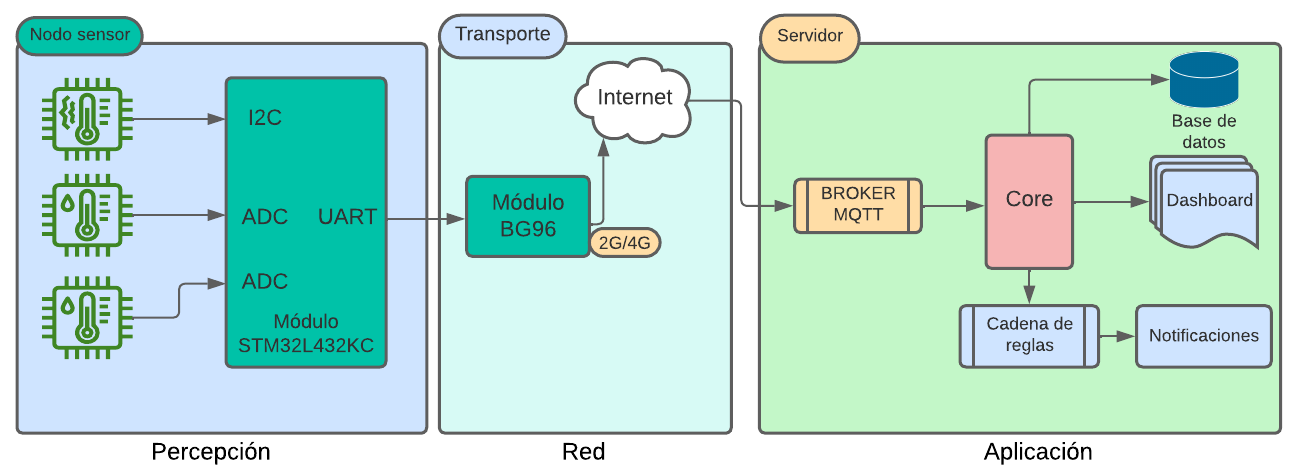
\includegraphics[width=1\textwidth]{./Figures/DiagramaDelSistema.png}
	\caption{Diagrama general del sistema IoT.}
	\label{fig:Diagrama general del sistema IoT}
\end{figure}

En cada una de las capas, se despliegan tecnologias y componentes de hardware y software. A continuación se describe cada una de ellas.

\begin{itemize}
	\item Capa de percepción. En la capa de percepción, los nodos sensores son los encargados de medir variables ambientales, hacer un prepocesamiento y enviarlas a la capa de red. Para su desarrollo se utilizo la placa STM32L432KC que contiene el firmware del sistema,tambien consta de un sensor de humedad y temperatrua ambiente AHT10 que se comunica con la placa de desarrollo mediante el protocolo I2C, sensor de humedad de suelo HL-69 y el sensor de luz UV ML-18 que se comunicacion con el modulo mediante entradas analogicas.
  \item Capa de red. En cuanto a la red, se utilizo un modulo quectel BG96 que puede conectarse a la red 2G, 4G, NB-IoT automaticamente dependiendo del nivel de la red en el lugar de la implementacion del modulo sensor, se comunica con el microcontrolador por comandos AT por puerto UART.
  \item Capa de aplicación. En la capa de aplicacion, se utilizo una plataforma IoT como servidor, que nos brinda las funcionalidades de broker MQTT para mandar los datos a la plataforma, base de datos para el almacenamiento, nos brinda la interfaz grafica para la visualizacion de los datos y nos permite gestionar la alarmas del sistema.


\end{itemize}

\section{Arquitectura de firmware}
\begin{verbatim}
  \begin{lstlisting}[caption= "un epígrafe descriptivo"]
    las líneas de código irían aquí...
  \end{lstlisting}
  \end{verbatim}

A modo de ejemplo:

\begin{lstlisting}[label=cod:vControl,caption=Pseudocódigo del lazo principal de control.]  % Start your code-block

#define MAX_SENSOR_NUMBER 3
#define MAX_ALARM_NUMBER  6
#define MAX_ACTUATOR_NUMBER 6

uint32_t sensorValue[MAX_SENSOR_NUMBER];		
FunctionalState alarmControl[MAX_ALARM_NUMBER];	//ENABLE or DISABLE
state_t alarmState[MAX_ALARM_NUMBER];						//ON or OFF
state_t actuatorState[MAX_ACTUATOR_NUMBER];			//ON or OFF

void vControl() {

	initGlobalVariables();
	
	period = 500 ms;
		
	while(1) {

		ticks = xTaskGetTickCount();
		
		updateSensors();
		
		updateAlarms();
		
		controlActuators();
		
		vTaskDelayUntil(&ticks, period);
	}
}
\end{lstlisting}



